%!TEX root = ../chapter05.tex 
%----------------------------------------------------------------------------------------
%	
%----------------------------------------------------------------------------------------
%----------------------------------------------------------------------------------------
%	 
%----------------------------------------------------------------------------------------

%----------------------------------------------------------------------------------------
%	EXERCICES
%----------------------------------------------------------------------------------------

 

\newpage 
\loadgeometry{widelayout}  
\pagestyle{scrheadings} % Print headers again  
\KOMAoptions{
	headwidth=textwithmarginpar,
	headsepline=true,
	headsepline= 0.5pt,
	footwidth=textwithmarginpar,
} 
\onehalfspacing
\section{Exercices Triplets pythagoriciens} 
\begin{exercise}\hfill 
	\begin{enumerate}[label=\alph*), leftmargin=*]
		\item \textbf{(Un classique de 3\ieme)}	Montrer que la différence des carrés de deux nombres entiers consécutifs est toujours un nombre impair.
		\item Choisir un nombre $b$ impair strictement supérieur à 3, et l'élever au carré.
		\item Trouver 2 nombres entiers consécutifs dont la différence des carrés est égale à $b^2$. 
	\end{enumerate}
\end{exercise}
\begin{tBox}
	Un triplet Pythagoricien est un triplet de trois nombres \textbf{entiers} $a\leqslant  b<c$ tels que $a^2+b^2=c^2$. 
\end{tBox} 
 \begin{example}[Nous faisons] Cherchons des triplets pythagoriciens $(a; 15; c)$ :
 	
 	\noindent \parbox[t]{0.3\linewidth}{
 		$\begin{WithArrows}
 			a^2+ 15^2 &\rule{0pt}{1.8em} = c^2\\
 			15^2&\rule{0pt}{1.8em} = c^2-a^2\\
 			225& \rule{0pt}{1.8em} =
 		\end{WithArrows}$  
 	}
 	\parbox[t]{0.65\linewidth}{
 		$\operatorname{diviseurs(225)}=\{
 		1; 3; 5; 9; \phantom{15; \qquad 25; \qquad 45 ; \qquad ;75; \qquad ; 225 } \}$  
 		\begin{description}
 			\item[$c-a=1$];\rule{0pt}{1.8em} $c+a=225$ :
 			\item[$c-a=3$];\rule{0pt}{1.8em} $c+a=\qquad$ :
 			\item[$c-a=5$];\rule{0pt}{1.8em} $c+a=\qquad$ :
 			\item[$c-a=9$];\rule{0pt}{1.8em} $c+a=\qquad$ :
 			\item[$c-a=15$];\rule{0pt}{1.8em} $c+a=\qquad$ : 
 		\end{description}
 	}
 \end{example} 
\begin{exercise}[À vous]\label{chapitre05:exercice:tripletspythagoriciens}   Combien pouvez vous trouver de triplets pythagoriciens $(a; 12; c)$ ?
\end{exercise} 
%\begin{eBox}
%	La tablette \href{https://en.wikipedia.org/wiki/Plimpton_322}{Plimpton 322} est la plus connue des  \numprint{500000} tablettes babyloniennes dans la collection G. A. Plimpton à l'université de Columbia. Rédigée dans de l'argile en 1800 av. J.-C., elle comporte un tableau de nombres rangés dans 4 colonnes et 15 lignes. Les valeurs des 3 premières colonnes sont associées à des triplets Pythagoriciens vérifiant $a^2+b^2=c^2$ (la 4\ieme étant le numéro de la ligne).  
%	
%	Une \href{https://www.maa.org/sites/default/files/pdf/upload_library/22/Ford/Robson105-120.pdf}{analyse minutieuse} a permis d'identifier la méthode utilisée pour obtenir chacune des lignes. Cet algorithme est abordé dans l'exercice suivant.
%\end{eBox}
\begin{exercise}[Comprendre la tablette Plimpton 322]\label{chapitre05:exercice:plimpton322}(figure \ref{chapter05:figure:plimpton322})\hfill  
	\begin{enumerate}[leftmargin=*,label=\alph*)]
		\item Montrer que pour toute valeur de $x>0$ le triangle ci-dessous est rectangle.
		
		%	\begin{figure*}[hb] 
		\noindent\parbox{1\linewidth}{\centering
			\begin{tikzpicture}[scale=.8]
				%			\tkzInit[xmin=-1.0,ymin=-1.0,xmax=6.5,ymax=2.8]
				%			\tkzClip
				\tkzDefPoint(0,0){A} \tkzDefPoint(5,0){C}
				\tkzDefTriangle[two angles = 27 and 90](A,C)\tkzGetPoint{B}
				\tkzDrawPolygon[line width=1.2pt](A,B,C) 
				\tkzLabelSegment[below](A,C){$2$}
				\tkzLabelSegment[right](B,C){$x-\frac{1}{x}$}
				\tkzLabelSegment[above left](A,B){$x+\frac{1}{x}$} 
			\end{tikzpicture}   
		}
		%	\end{figure*}  
		\item Expliquer pourquoi cette figure illustre l'inégalité pour tout $x> 0$ on a $2\leqslant x+\frac{1}{x}$.
		\item Donner, sous forme de fractions irréductibles, les longueurs des côtés du triangle rectangle correspondant à la valeur  $x=\tfrac{12}{5}$.
		
		Vérifier qu'il est semblable au triangle de côtés $169\colon 119\colon 120$ (1\iere ligne de la tablette).
		\item Même question pour $x=\tfrac{9}{4}$  et le triangle $97\colon 65\colon 72$ (11\ieme ligne de la tablette).
		\item Pouvez vous retrouver les triplets $(a;b;c)$ de la seconde ligne, qui correspond à $x=\tfrac{64}{27}$ ?
	\end{enumerate} 
\end{exercise} 
\begin{exercise}  
Les formules particulières suivantes génèrent des triplets pythagoriciens $(a;b;c)$ : 
%\setlength{\abovedisplayskip}{5pt}
%\setlength{\belowdisplayskip}{5pt}
%\begin{equation}
%\label{formules:tripletspythagore}

$
p;q\in\mathbb{N} \qquad a=p^2-q^2 \qquad b = 2 pq \qquad c = p^2+q^2 
$
%\end{equation} 
	\begin{enumerate}[label=\alph*), leftmargin=*]
		\item Donner le triplet correspondant à $(p=8;q=7)$ et vérifier l'égalité $a^2+b^2=c^2$ 
		\item Retrouver le couple d'entiers $(p;q)$ qui donnent le triplet $(a=35;b=12;c=37)$. 
		\item Développer, réduire et montrer que pour tout $p,q\in\mathbb{N}$ : $a^2+b^2=p^4+2p^2q^2+q^4$.
		\item  Montrer que pour tout $p,q\in\mathbb{N}$, on a  $a^2+b^2=c^2$.
	\end{enumerate}
\end{exercise}
 
%----------------------------------------------------------------------------------------
%	 
%----------------------------------------------------------------------------------------

 \newpage  
\begin{exercise}\label{chapitre05:exercice:tripletspythagoriciensAlgorithme}\hfill 
	
	\begin{enumerate}[label=\arabic*),leftmargin=*]
		\item Voici 3 scripts Python. Cocher les cases correspondant aux scripts qui affichent le couple indiqué :
		\begin{multicols}{2} \setlength\columnseprule{.0pt}
\begin{lstlisting}[ language=python , 
title=Script A,   
linewidth=1\columnwidth,
style=python-code,    
aboveskip=0.2\topskip,
belowskip=0.2\topskip,
%xleftmargin=1.2em,
lineskip=1.1em,
tabsize=4, 
numbers=none,
%	firstnumber=10  
]
for a in range(100) :
	for b in range(100) :
		print(a,b) 
\end{lstlisting}  
\begin{lstlisting}[ language=python , 
title=Script B,   
linewidth=1\columnwidth,
style=python-code,    
aboveskip=0.2\topskip,
belowskip=0.2\topskip,
%xleftmargin=1.2em,
lineskip=1.1em,
tabsize=4, 
numbers=none,
%	firstnumber=10  
] 
for a in range(100) :
	for b in range(a,100-a) :
		print(a,b) 
		
\end{lstlisting} 

\begin{lstlisting}[ language=python , 
title=Script C,   
linewidth=1\columnwidth,
style=python-code,    
aboveskip=0.2\topskip,
belowskip=0.2\topskip,
%xleftmargin=1.2em,
lineskip=1.1em,
tabsize=4, 
numbers=none,
	%	firstnumber=10  
	] 
for a in range(100) :
	b = 100 - a
	print(a,b)
\end{lstlisting}
\begin{lstlisting}[ language=python , 
title=Script D,   
linewidth=1\columnwidth,
style=python-code,    
aboveskip=0.2\topskip,
belowskip=0.2\topskip,
%xleftmargin=1.2em,
lineskip=1.1em,
tabsize=4, 
numbers=none,
	%	firstnumber=10  
	] 
for a in range(100) :
	for b in range(a,100) :
		if a**2+b**2 == 10**2 :
			print(a,b)  
\end{lstlisting}
		\end{multicols}
			 
\noindent \QCM[Multiple,Alterne,Reponses=4,Stretch=1.1,Largeur=3.0cm,%Solution,%
Noms={Script A/Script B/Script C/Script D}]{%\textbb{N} marche pas
{\lstinline|0, 10|} &1&1&0&1, 
{\lstinline|10, 0|} &1&0&0&0, 
{\lstinline|1, 99|} &1&0&1&0,
{\lstinline|3, 7|} &1&1&0&0, 
{\lstinline|4, 3|} &1&0&0&0, 
{\lstinline|6, 8|} &1&1&0&1,  
{\lstinline|8, 6|} &1&0&0&0, 
%{\lstinline|36, 64|} &1&0&1&0,
{\lstinline|75, 25|} &1&0&1&0, 
} 
\vfill 
		\item On cherche les triplets pythagoriciens $(a,b,c)$ correspondant à des triangles de périmètre 1000.
 
\noindent \begin{lstlisting}[ language=python , 
%	title=Script D,   
	linewidth=1\columnwidth,
	style=python-code,    
	aboveskip=0.2\topskip,
	belowskip=0.2\topskip,
	%xleftmargin=1.2em,
	lineskip=1.1em,
	tabsize=4, 
	numbers=none,
	%	firstnumber=10  
	] 
for a in ................       :
	for b in ................   :
		c = ...................
		if .................... :
			print(a,b,c)
\end{lstlisting} 
\begin{enumerate}[label=\alph*),leftmargin=*]
	\item Expliquer pourquoi $a$, $b$ et $c$ sont forcement inférieurs à 1000.
	\item Compléter le script ci-dessous afin qu'il affiche les bons triplets.
	\item Rentrer le script sur votre pythonette et l'exécuter. \\
	Vérifier qu'il n'affiche aucune valeur négative. puis relever les triplets solutions.
\end{enumerate} 
\end{enumerate}
\end{exercise}
%----------------------------------------------------------------------------------------
%	 
%----------------------------------------------------------------------------------------

\newpage 
\begin{proof}[solution de l'exemple et de l'exercice \ref{chapitre05:exercice:tripletspythagoriciens}]\hfill  
	\begin{enumerate}[label=\alph*),leftmargin=*]
		\item Pour $b=15$ on trouve $117^2+15^2=118^2$, $36^2+15^2=39^2$, $20^2+15^2=25^2$ et $8^2+15^2=17^2$.
		\item Pour $b=12$ on trouve $35^2+12^2=37^2$, $16^2+12^2=20^2$, $9^2+12^2=15^2$ et $5^2+12^2=13^2$. 
	\end{enumerate}
\end{proof}
 \begin{figure*}[hb]
	\includegraphics[width=0.60\linewidth]{Plimpton322-Drawing by Eleanor Robson.png} 
	\caption{La tablette \href{https://en.wikipedia.org/wiki/Plimpton_322}{Plimpton 322} est la plus connue des  \numprint{500000} tablettes babyloniennes dans la collection G. A. Plimpton à l'université de Columbia. Rédigée dans de l'argile en 1800 av. J.-C., elle comporte un tableau de nombres rangés dans 4 colonnes et 15 lignes. Les valeurs des 3 premières colonnes sont associées à des triplets pythagoriciens vérifiant $a^2+b^2=c^2$ (la 4\ieme étant le numéro de la ligne).  
	Une \href{https://www.maa.org/sites/default/files/pdf/upload_library/22/Ford/Robson105-120.pdf}{analyse minutieuse} a permis d'identifier la méthode utilisée pour obtenir chacune des lignes. Cet algorithme est abordé dans l'exercice \ref{chapitre05:exercice:plimpton322}.}\label{chapter05:figure:plimpton322}
\end{figure*} 
\begin{proof}[solution de l'exercice \ref{chapitre05:exercice:tripletspythagoriciensAlgorithme}]\hfill  
	
\noindent \QCM[Multiple,Alterne,Reponses=4,Stretch=1.0,Largeur=3.0cm,Solution,%
Noms={Script A/Script B/Script C/Script D}]{%\textbb{N} marche pas
	{\lstinline|0, 10|} &1&1&0&1, 
	{\lstinline|10, 0|} &1&0&0&0, 
	{\lstinline|1, 99|} &1&0&1&0,
	{\lstinline|3, 7|} &1&1&0&0, 
	{\lstinline|4, 3|} &1&0&0&0, 
	{\lstinline|6, 8|} &1&1&0&1,  
	{\lstinline|8, 6|} &1&0&0&0, 
	%{\lstinline|36, 64|} &1&0&1&0,
	{\lstinline|75, 25|} &1&0&1&0, 
} 

\begin{lstlisting}[ language=python , 
	%	title=Script D,   
	linewidth=1\columnwidth,
	style=python-code,    
	aboveskip=0.2\topskip,
	belowskip=0.2\topskip,
	%xleftmargin=1.2em,
%	lineskip=1.0em,
	tabsize=4, 
	numbers=none,
	%	firstnumber=10  
	] 
for a in range(1000) :
	for b in range(a,1000-a)  :
		c = 1000 - a - b
		if a**2 + b**2 == c**2 :
			print(a,b,c)				# programme affiche 200, 375, 475
\end{lstlisting} 
\end{proof}